%%%%%%%%%%%%%%%%%%%%%%%%%%%%%%%%%%%%%%%%%%%%%%%%%%%%%%%%%%%%%%%%%%%%%%%%
%    INSTITUTE OF PHYSICS PUBLISHING                                   %
%                                                                      %
%   `Preparing an article for publication in an Institute of Physics   %
%    Publishing journal using LaTeX'                                   %
%                                                                      %
%    LaTeX source code `ioplau2e.tex' used to generate `author         %
%    guidelines', the documentation explaining and demonstrating use   %
%    of the Institute of Physics Publishing LaTeX preprint files       %
%    `iopart.cls, iopart12.clo and iopart10.clo'.                      %
%                                                                      %
%    `ioplau2e.tex' itself uses LaTeX with `iopart.cls'                %
%                                                                      %
%%%%%%%%%%%%%%%%%%%%%%%%%%%%%%%%%%
%
%
% First we have a character check
%
% ! exclamation mark    " double quote  
% # hash                ` opening quote (grave)
% & ampersand           ' closing quote (acute)
% $ dollar              % percent       
% ( open parenthesis    ) close paren.  
% - hyphen              = equals sign
% | vertical bar        ~ tilde         
% @ at sign             _ underscore
% { open curly brace    } close curly   
% [ open square         ] close square bracket
% + plus sign           ; semi-colon    
% * asterisk            : colon
% < open angle bracket  > close angle   
% , comma               . full stop
% ? question mark       / forward slash 
% \ backslash           ^ circumflex
%
% ABCDEFGHIJKLMNOPQRSTUVWXYZ 
% abcdefghijklmnopqrstuvwxyz 
% 1234567890
%
%%%%%%%%%%%%%%%%%%%%%%%%%%%%%%%%%%%%%%%%%%%%%%%%%%%%%%%%%%%%%%%%%%%
%
\documentclass[12pt]{iopart}
\bibliographystyle{iopart-num_custom}
\usepackage{xcolor}
\usepackage{pifont}
\usepackage{comment}
\usepackage{acronym}
\usepackage{standalone}
\usepackage{academicons}
\usepackage{scalerel}
\usepackage{layouts}
%\usepackage{import}
\usepackage{subfig}
\usepackage{tikz}
\usetikzlibrary{decorations.pathreplacing,angles,quotes,shapes.geometric, arrows,calc}
\usetikzlibrary{svg.path}
\expandafter\let\csname equation*\endcsname\relax 
\expandafter\let\csname endequation*\endcsname\relax 
\usepackage{amsmath}
\usepackage{amssymb}
\usepackage{hyperref}
\usepackage[capitalize]{cleveref}
\newcommand{\gguide}{{\it Preparing graphics for IOP Publishing journals}}
%Uncomment next line if AMS fonts required
%\usepackage{iopams}  
\newcommand{\jordan}[1]{\textbf{\textcolor{red}{JORDAN: #1}}}
\newcommand{\siong}[1]{\textbf{\textcolor{blue}{SIONG: #1}}}
\newcommand{\chris}[1]{\textbf{\textcolor{green}{CHRIS: #1}}}
\newcommand{\michael}[1]{\textbf{\textcolor{orange}{MICHAEL: #1}}}
\newcommand{\dcc}{LIGO-PXXXXXXX}
%\input{tag.tex}
% Command for ORCID id's
\definecolor{orcidlogocol}{HTML}{A6CE39}
\tikzset{
  orcidlogo/.pic={
    \fill[orcidlogocol] svg{M256,128c0,70.7-57.3,128-128,128C57.3,256,0,198.7,0,128C0,57.3,57.3,0,128,0C198.7,0,256,57.3,256,128z};
    \fill[white] svg{M86.3,186.2H70.9V79.1h15.4v48.4V186.2z}
                 svg{M108.9,79.1h41.6c39.6,0,57,28.3,57,53.6c0,27.5-21.5,53.6-56.8,53.6h-41.8V79.1z M124.3,172.4h24.5c34.9,0,42.9-26.5,42.9-39.7c0-21.5-13.7-39.7-43.7-39.7h-23.7V172.4z}
                 svg{M88.7,56.8c0,5.5-4.5,10.1-10.1,10.1c-5.6,0-10.1-4.6-10.1-10.1c0-5.6,4.5-10.1,10.1-10.1C84.2,46.7,88.7,51.3,88.7,56.8z};
  }
}

\newcommand\orcidicon[1]{\href{https://orcid.org/#1}{\mbox{\scalerel*{
\begin{tikzpicture}[yscale=-1,transform shape]
\pic{orcidlogo};
\end{tikzpicture}
}{|}}}}

\usepackage{hyperref} %<--- Load after everything else

\begin{document}

\title{Generalised gravitational burst generation with Generative Adversarial Networks}

\author{
    J. McGinn \orcidicon{0000-0000-0000-0000},
    C. Messenger \orcidicon{0000-0001-7488-5022},
    I.S. Heng \orcidicon{0000-0000-0000-0000},
    M. J. Williams \orcidicon{0000-0003-2198-2974}
}

\address{University of Glasgow, Physics \& Astronomy Department, Glasgow G12 8QQ, UK}
%\ead{jordan.mcginn@glasgow.ac.uk}
\vspace{10pt}
%\begin{indented}
%\item[]\commitDATE\\\mbox{\small \commitID}\\\mbox{\dcc}
%\end{indented}

\begin{abstract}
The next generation of Gravitational wave detectors will accelerate the number
of gravitational wave detection's such that we can gain new in site into the
physics behind the sources causing the phenomena. Numerical simulations and
matched filtering are the standard for detecting gravitational waves for know
sources such as binary-black hole mergers. Other sources of gravitational waves
that remain elusive to standard modelling techniques and are expected to be
detectable, however, there must be a way to characterise them in order to build
a model template. Here we construct a unmodeled burst generation scheme using
Generative adversarial networks - a powerful class of machine learning.
\end{abstract}

%
% Uncomment for keywords
%\vspace{2pc}
%\noindent{\it Keywords}: XXXXXX, YYYYYYYY, ZZZZZZZZZ
%
% Uncomment for Submitted to journal title message
%\submitto{\JPA}
%
% Uncomment if a separate title page is required
%\maketitle
% 
% For two-column output uncomment the next line and choose [10pt] rather than [12pt] in the \documentclass declaration
%\ioptwocol
%

\acrodef{GW}[GW]{Gravitational wave}
\acrodef{GAN}[GAN]{generative adversarial network}
\acrodef{CGAN}[CGAN]{conditional generative adversarial network}
\acrodef{ACGAN}[ACGAN]{auxilliary conditional generative adversarial network}
\acrodef{DCGAN}[DCGAN]{deep convolutional generative adversarial network}
\acrodef{CNN}[CNN]{convolutional neural networks}
\acrodef{BBH}[BBH]{binary black hole}


\section{Introduction}
%textwidth in inches: \printinunitsof{in}\prntlen{\textwidth}
\begin{comment}
\begin{itemize}
\item Need to introduce GWs - the current state of the field e.g. detections
and LVC papers \ding{51}
\item Introduce burst searches - what's the point of burst searches \ding{51} - lots of references 
\item Discuss the family of burst waveforms currently used and why - not in detail, just
an introduction \ding{51}
\item Introduce ML techniques in GWs \ding{51} - lots of references
\item What this paper does on GANs in 1 paragraph \ding{51}
\item Describe the structure of the paper 
\end{itemize}
\end{comment}

% introduce \ac{GW} astrophsyics
%
Gravitational wave astronomy is now an established field, starting with the first
detection of a binary black hole merger \cite{Abbott2016} in September 2015.
Following this, the first and second observations runs (O1 and O2) of Advanced
LIGO and Advanced Virgo \cite{Prospects-dets, AdvLIGO, AdvLIGO2, AdvVIRGO} reported several more Compact Binary Coalescence (CBC)
mergers \cite{Abbott2016a, Abbott2017, Abbott2017a, Abbott2017b}. On August
2017 a binary neutron star merger was observed alongside its electromagnetic
counterpart for the first time, giving rise to multimessenger gravitational
wave astronomy. 

% introduce burst searches
%
With these successes and continued upgrades to the detectors, further detections of CBCs are expected to be commonplace in a few short years. Another group of GW signals that has thus far been undetectable is GW ``bursts".  GW bursts are transient signals of typically short duration ($<$ 1s) whose
waveforms are not accurately modelled or are complex to re-produce.
Astrophysical sources for such transients include: Core collapse supernova \cite{Fryer_2003}, Pulsar glitches \cite{Andersson_2001}, Neutron star
post-mergers \cite{Baiotti_2007} and other as-yet unexplained physical phenomena. 

GW detections so far have used a process called matched filtering, \cite{Owen1998}, where a large template bank of possible GW waveforms are compared to the detector outputs. In order to increase the chances of detection these template banks must span a large multi dimensional parameter space and the templates must be accurate, requiring significant computational cost.  GW bursts are un-modelled; therefore there are no templates available and so these signals are undetectable through this scheme. Instead, detection involves distinguishing
the signal from detector noise. Burst searches look for excess power contained in the time-frequency domain and rely on the astrophysical burst waveform appearing in multiple detectors at similar times. This is only possible if the detector noise is
well characterised and the candidate signal can be differentiated from
systematic or environmental glitches. 

% Discuss the family of burst waveforms currently used and why - not in detail, just
% an introduction 
%
\ac{GW} burst algorithms \cite{Klimenko_2008, Aso_2008} are tested and tuned using model waveforms that may
or may not have astrophysical significance but have easy to define parameters
and share characteristics of real bursts that is enough to simulate a \ac{GW} passing between detectors. Such waveforms include sine-Gaussians: a Gaussian modulated sine wave that is by it's central frequency and decay parameter. Bandlimited white-noise bursts: white noise that is contained within a certain frequency range and ring-downs which mimic the damped oscillations after a CBC merger.

\begin{comment}Such waveforms may have
long-duration, short bandwidth (ringdowns), long-duration, large bandwidth
(inspirals) and many algorithms make use of sine-Gaussians: a Gaussian
modulated sine wave that is characterised by it's central frequency and narrow
bandwidth.~\chris{not the time to try to describe the types of burst waveforms.
Also, be careful with satying things like ringdowns have narrow bandwidth. I
know we specify a single frequency but becuase of the short duration, the
signal is broad band. Look at the FFT} This makes it a great tool for
diagnosing LIGOs sensitivity to frequency.~\chris{strange unfinished sentence.} 
\end{comment}

% Introduce ML techniques in GWs
%

With the expectation that there will be many more \ac{GW} detections in the future, researches are starting to realise the need for fast and efficient \ac{GW} analysis to compete with the rising number of detections. While still in its infancy, Machine Learning (ML) with GW has already shown great potential for overcoming data bottlenecks. \ac{GW} analysis in areas of detection \cite{Gabbard2017,Gebhard_2019,Krastev_2020}, glitch classification \cite{Bahaadini, George_2018,Razzano_2018} and parameter estimation \cite{gabbard2019bayesian,shen2019deterministic,green2020gravitationalwave} have shown the success of in ML pattern recognition. Applying these algorithms show similar results to matched filtering techniques and have the benefit of being orders of magnitude faster. 

% What this paper does on GANs in 1 paragraph
%

In this work we aim to explore the use of machine learning to generate and interpret
unmodelled \ac{GW} burst waveforms. Using the generative machine learning model: Generative Adversarial Networks (GANs), we train on five classes of known burst morphologies in the time domain. Working on the assumption that GANs construct smooth n-dimension vector spaces between it's input and output, we can then explore the space between the five classes to construct new unmodelled waveforms. As all the computationally expensive processes occur during training, the learned model after training is able to produce waveforms much faster than and in fact produce waveforms that are impossible to produce with current techniques. These new varieties of waveforms can then be used to diagnose detection algorithms and gain new insight into sources of \ac{GW} bursts. 
% the point of the paper
%

This paper is organised as follows: \jordan{unstructured at the moment}


%%%%%%%%%%%%%%%%%%%%%%%%%%%%%%%%%%%%%%%%%%%%%%%%%%%%%%%%%%%%%%%%%%%%%%%%%%%%%%
\section{Generative Adversarial Networks}
%%%%%%%%%%%%%%%%%%%%%%%%%%%%%%%%%%%%%%%%%%%%%%%%%%%%%%%%%%%%%%%%%%%%%%%%%%%%%%

\begin{comment}
\begin{itemize}
\item Describe GANs in detail but really focus on the fact that the reader is a
GW data analyst - not a computer scientist \ding{51}
\item A diagram would be very useful \ding{51}
\item Do not discuss our specific case here - just stay general \ding{51}
\item A subsection on the specific advanced flavour of GAN that you are using
here - motivate this choice. \ding{51}
\end{itemize}
\end{comment}

% introduce GANs
%
\subsection{Artificial neural networks}

\begin{figure}
    \begin{minipage}[b]{0.3\linewidth}
        \subfloat[]{\label{fig:perceptron}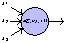
\includegraphics[width=\linewidth,height=0.65\linewidth]{figures/neural_network-figure0.pdf}}
        \par
        \vspace{\baselineskip}
        \subfloat[]{\label{fig:tanh_activation}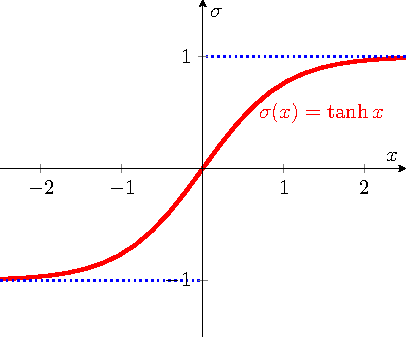
\includegraphics[width=\linewidth,height=0.65\linewidth]{figures/neural_network-figure1.pdf}}
    \end{minipage}
        \begin{minipage}[b]{0.7\linewidth}
        \subfloat[]{\label{fig:neural_network}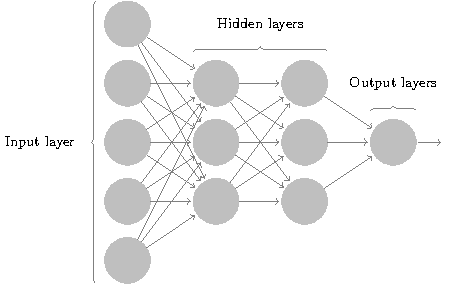
\includegraphics[width=\linewidth,height=0.65\linewidth]{figures/neural_network-figure2.pdf}}
    \end{minipage}
    \caption{Neural Networks (a) A single neuron taking a vector of inputs and returning a singular output based on the weights, bias and activation function of the network. (b) The hyperbolic tangent used as an activation function. (c) A fully connected neural network containing two hidden layers that performs a mapping of an input vector to a singular output. \michael{Equation in the neuron looks very small}}
\end{figure}

Since the birth of programmable computers, people have wondered if machines can develop true intelligence beyond formal mathematical procedures. Today, ML aims to learn apparent relationships held within the given data or `training data' in order to make accurate predictions without the need for additional programming . A common approach in ML relies on the computer learning on past experience to make decisions on future events. The hierarchical nature of this approach means that the machine can build complicated concepts from simpler ones. This branch of AI is called deep learning.
Neural networks are the quintessential machine learning algorithm that aims to approximate a function. They are built from many single processing units called neurons. The simpliest Neural Network is the perceptron layer \cref{fig:perceptron} which holds a single neuron that takes several real inputs $x_{1}, ... , x_{i}$ and maps them to an output according to the following linear equation: 

\begin{equation}
\sigma(\sum_i w_i x_i + b),
\label{eqn:neuron}
\end{equation}
where $w$ and $b$ are the weights and bias and $\sigma$ denotes the activation function. The weights are numbers which can be thought as the strength between connections. The output of a neuron is called its activation. Different choices of activation functions allow the user to simulate various models. A common example of an activation function is the hyperbolic tangent \cref{fig:tanh_activation} that is used when the outputs of the network must be both positive and negative and re-scaled to $[-1,1]$. It is often useful to introduce a bias, $b$, such that the neuron remains inactive above zero but is active when the sum reaches a defined threshold. This bias is added before the activation function and it tells us how high the weighted sum needs to be before the neuron becomes active.

The output of a single neuron is defined by \cref{eqn:neuron} and gives a prediction $\hat{y}$ that can be compared to the real value $y$ through a cost or loss function. If the loss is non-zero, the network must work to minimise this function by updating the weights in the negative direction of the loss gradient in a process referred to as gradient descent. This loss function plays a critical role in how neural networks learn.

A neural network contains many single neurons connected in a layered structure as shown in \cref{fig:neural_network}. The activations of the first layer (or input layer) act as the inputs to the second layer and so on until the output layer. Multilayered neural networks have intermediate layers between the input and output stages dubbed the hidden layers as the computations performed are not accessible to the user. The network can be thought of as a function F: $\mathbb{R}^N\rightarrow \mathbb{R}^M $ reliant on how activations from one layer bring activations in the next. The system is analogous to biology, where, some groups of neurons in animal brains cause certain others to fire. 

\subsection{Convolutional Neural Networks}
Convolutional Neural Networks (CNNs) are designed to work with grid-like structures that exhibit strong local spatial dependencies. An example would be a two-dimensional image as each coloured pixel has similar intensities to their near neighbours. The value contained in each pixel can be thought of as adding an additional dimension or channel to the image. Although most work with CNNs involve image-based data, they can be applied to other spatially adjacent data types such as time-series and text items. CNNs are defined by the use of a convolution operation, a mathematical operation that expresses the amount overlap between functions. The convolution is applied by shifting one grid-like structure over the other, drawing out spatially important features between the two.  A strided convolution reduces the dimensionality of the input while retaining spatial features. This can result in a loss of information along the boarders. To combat this, the input is padded with zeros at the edges which does not interfere with the convolutional operation. The output of the convolutional layer is then passed to an activation function. 

\subsection{GANs}

A subset of deep learning that has seen fruitful development in recent years is \acp{GAN} \cite{Goodfellow2014}. These unsupervised algorithms learn
patterns in a given training data set using an adversarial process. The
generations from \acp{GAN} are state-of-the-art in fields such as high quality image
fidelity \cite{brock2018large,karras2019analyzing}, text-to-image translation
\cite{reed2016generative} and video prediction \cite{liang2017dual} as well as
time series generations \cite{esteban2017realvalued}. 

% How a GAN works
%
\acp{GAN} train two competing neural networks, consisting of a discriminator
that is set up to distinguish between real and fake data and a generator that
produces synthetic reproductions of the real data. The generator performs a
mapping from an input noise vector $\mathbf{z}$, that is usually sampled from a n-dimensional Gaussian space known as the latent space, to its representation of the
data and the discriminator maps its input $\mathbf{x}$ to a probability that
the input came form either the training data or generator.  During training,
the discriminator is given a batch of samples that contains one half real data
and one half fake data which it then makes predictions on. The loss for the
discriminator is calculated by comparing its predictions to the labelled data
through the binary cross-entropy function. \jordan{note to myself: This is important since eqn 2 is derived from it (thats where the logs come from)} The training process of a \ac{GAN}
alternatively updates the weights of the discriminator and generator based on
information on its competitors loss function. This loss of discriminator is
used to update the weights of the generator to produce more realistic samples
of the input distribution, the loss of the generator encourages the
discriminator to update its classification abilities. GANs seek to find an equilibrium between the generator and discriminator in the form of a two-player game that can be summarised by the following:  

\begin{comment}
Both networks compete in
a minimax game~\chris{what is a minimax game? references?} which the generator
is trying to minimise and the discriminator is trying to
maximise:~\chris{nicely written, however, it needs an extra 25\% explanation
for people not familar with ML or GANs in particular. Try to spell things out
more. Also refer to Fig 1 somewhere in this section.}
\end{comment}
%
\begin{equation}
  \mathop{\text{min}}_{G}  \mathop{\text{max}}_{D} V(D,G) = \mathbb{E}_{\mathbf{x} \sim p_{\text{r}}(\mathbf{x})} [\text{log} D(\mathbf{x})] \\ + \mathbb{E}_{\mathbf{z} \sim p_{\text{z}}(\mathbf{z})} [\text{log}(1-D(G(\mathbf{z})))],
\label{equation:GANloss}
\end{equation}

where, V is an objective function that is to be optimized. Objective functions are a general term for either a loss function (to be minimized) or a negative loss function (to be maximised). D is the discriminator, G is the generator and ${\mathbf{x} \sim p_{\text{r}}(\mathbf{x})}$, ${\mathbf{z} \sim p_{\text{z}}(\mathbf{z})}$ are samples taken from the training data and generated data respectfully. In practice this approach was found to be unstable. Early on in training the generators weights are initialised randomly meaning that the early generations are noisy and uninformative. This means that the discriminator can easily learn to spot the fake generations and so the discriminator wins and the generator cannot continue to improve. To overcome this the framing of the generator is often changed. Rather than minimizing $\text{log}(1-D(G(\mathbf{z})))$ the objective now is to maximise $\text{log}(D(G(\mathbf{z})))$, that is, to maximise the probability of the generations being predicted as real. The idea being that we always want the loosing side to be able to leverage from its competitor. 
%

% describing the problems with GANs 
%
In theory, the adversarial process will eventually lead to the local Nash
equilibrium \cite{Nash1950} whereby both neural networks are trained
optimally. In practice, however, \acp{GAN} are notoriously difficult
to train. Such difficulties include: Non-convergence, where the model
parameters oscillate and the loss never converges, mode collapse where the generator produces a
limited diversity of samples, and diminishing
gradients when applying gradient descent to a loss function that is discontinuous.

\subsection{Conditional GANs}

% introduce CGANs and ACGANs
%
To gain more control over what a GAN is able to generate, a conditional variant of \acp{GAN} named \acp{CGAN}~\cite{cgan} was introduced by feeding in extra information into the generator and discriminator such as a class label or attribute label, c. The objective function is then modified:
\begin{equation}
  \mathop{\text{min}}_{G}  \mathop{\text{max}}_{D} V(D,G) = \mathbb{E}_{\mathbf{x,c} \sim p_{\text{r}}(\mathbf{x,c})} [\text{log} D(\mathbf{x,c})] \\ + \mathbb{E}_{\mathbf{z} \sim p_{\text{z}}(\mathbf{z}),\mathbf{c} \sim p_{\text{r}}(\mathbf{c})} [\text{log}(1-D(G(\mathbf{z,c})))].
\label{equation:cGANloss}
\end{equation}

This simple addition has shown to work well in practice, for instance in image-to-image translation \cite{isola2016imagetoimage}. We will be using a conditional GAN for this study.
%
\begin{comment}adds structure to the latent space by providing the
generator with a class or attribute label. The generator learns to segment the
latent space by clustering distributions which have similar properties, making
a point in latent space conditional on a class~\chris{are we sure about this?
all classes share the same latent space and I don't think that the space gets
segmented into areas corresponding to different classes - I do think that it
gets broken down into spaces with different intrinsic physical properties e.g.,
high frequency, long duration, etc...}.
\end{comment}
%
\begin{comment}
This idea was extended further with
\acp{ACGAN}~\cite{odena2016conditional} that require the discriminator to
output a probability of data belonging to each class. A pictorial
representation on the differences between these approaches is shown in
Fig.~\ref{fig:gan_comparison} \jordan{self note: Probably move away from ACGAN part, standalone aux classifiers can be trained later if that's what you want}. 
\end{comment}

\begin{figure}
    \centering
        %\documentclass{article}
%\usepackage{comment}
%\usepackage{tikz}
%\usetikzlibrary{shapes.geometric, arrows, calc}

%\begin{document}
    
\begin{tikzpicture}[node distance=2cm]

\tikzstyle{zinput} = [rectangle, rounded corners, text centered, draw=black]%, fill=red!30]
\tikzstyle{generator} = [rectangle, rounded corners, text centered, draw=black]%, fill=red!30]
\tikzstyle{X real} = [rectangle, rounded corners, text centered, draw=black]%, fill=red!30]
\tikzstyle{X fake} = [rectangle, rounded corners, text centered, draw=black]%, fill=red!30]
\tikzstyle{X real} = [rectangle, rounded corners, text centered, draw=black]%, fill=red!30]
\tikzstyle{discriminator} = [rectangle, rounded corners, text centered, draw=black]%, fill=red!30]
\tikzstyle{real/fake} = [rectangle, rounded corners, text centered, draw=black]%, fill=red!30]

\tikzstyle{arrow} = [thick,->,>=stealth]

\node (r) [X real] {\textbf{X} real};
\node (f) [X fake, right of = r] {\textbf{X} fake};
\node (G) [generator,above of = f, scale = 2] {\textbf{G}};
\node (z) [zinput] [zinput, above of = G] {\textbf{z} (noise)};
\node (D) [discriminator, below of = f, xshift = -1cm, scale = 2] {\textbf{D}};
\node (rf) [real/fake, below of = D] {real/fake};

\draw [arrow] (z) -- (G);
\draw [arrow] (G) -- (f);
\draw [arrow] (r) edge[out=270,in=90] (D);
\draw [arrow] (f) edge[out=270,in=90] (D);
\draw [arrow] (D) -- (rf);

\end{tikzpicture}
%\end{document}
%     without .tex extension
        \begin{tikzpicture}[node distance=2cm]

\tikzstyle{zinput} = [rectangle, rounded corners, text centered, draw=black]%, fill=red!30]
\tikzstyle{generator} = [rectangle, rounded corners, text centered, draw=black]%, fill=red!30]
\tikzstyle{X real} = [rectangle, rounded corners, text centered, draw=black]%, fill=red!30]
\tikzstyle{X fake} = [rectangle, rounded corners, text centered, draw=black]%, fill=red!30]
\tikzstyle{X real} = [rectangle, rounded corners, text centered, draw=black]%, fill=red!30]
\tikzstyle{discriminator} = [rectangle, rounded corners, text centered, draw=black]%, fill=red!30]
\tikzstyle{real/fake} = [rectangle, rounded corners, text centered, draw=black]%, fill=red!30]
\tikzstyle{coutput} = [rectangle, rounded corners, text centered, draw=black]%, fill=red!30]

\tikzstyle{arrow} = [thick,->,>=stealth]

\node (r) [X real] {\textbf{X} real};
\node (f) [X fake, right of = r, xshift = 0cm] {\textbf{X} fake};
\node (G) [generator,above of = f, scale = 2] {\textbf{G}};
\node (z) [zinput] [zinput, above of = G, xshift = 1cm] {\textbf{z} (noise)};
\node (c) [coutput, left of = z] {\textbf{c} (class)};
\node (D) [discriminator, below of = f, xshift = -1cm, scale = 2] {\textbf{D}};
\node (rf) [real/fake, below of = D] {real/fake};
%\node (co) [coutput, left of = rf, xshift = -0.5cm] {c = 1, 2, ...};

\draw [arrow] (z) edge[out=270,in=90] (G);
\draw [arrow] (c) edge[out=270,in=90] (D);
\draw [arrow] (c) edge[out=270,in=90] (G);
\draw [arrow] (c) edge[out=270,in=90] (r);
\draw [arrow] (G) -- (f);
\draw [arrow] (r) edge[out=270,in=90] (D);
\draw [arrow] (f) edge[out=270,in=90] (D);
\draw [arrow] (D) edge[out=270,in=90] (rf);
%\draw [arrow] (D) edge[out=270,in=90] (co);

\end{tikzpicture}%     without .tex extension
    \caption{Comparison of the original GAN method and the
Conditional-GAN method. For CGANs the training data requires a label denoting
its class that is also fed to the generator which then learns to generate
waveforms based on the input label.} \label{fig:gan_comparison}
\end{figure}

%%%%%%%%%%%%%%%%%%%%%%%%%%%%%%%%%%%%%%%%%%%%%%%%%%%%%%%%%%%%%%%%%%%%%%%%%%%%%%
\section{Methodology}
%%%%%%%%%%%%%%%%%%%%%%%%%%%%%%%%%%%%%%%%%%%%%%%%%%%%%%%%%%%%%%%%%%%%%%%%%%%%%%

\begin{comment}
\begin{itemize}
\item Need to introduce the scheme you propose to use
\item A paragraph or subsection on the data generation being very clear on all
5 waveform models and the prior parameter space for each \ding{51}
\item A subsection on the design of the network architecture \ding{51}
\item A subsection on the "box" and why we implement it \ding{51}
\item A subsection on the training of the network - give rough timings and rule
of thumb decisions made
\item Do not discuss the results here 
\end{itemize}
\end{comment}

% introduce the training data
%

\begin{table}[hb]
\centering
\caption{Burst training parameters}
%\footnotesize
\begin{tabular}{@{} l l l l l l }
\br
\hline
 Waveform & Central frequency  & Decay & Central time epoch & Mass range \\
 & (Hz) & (s) & (s) & ($\textrm{M}_{\odot}$) \\
\mr
Sine-Gaussian & 70 - 250 & 0.004 - 0.03 & 0.4 - 0.6 & N/A  \\  
Ringdown & 70 - 250 & 0.004 - 0.03 & 0.4 - 0.6 & N/A \\
White-noise burst & 70 - 250 & 0.004 - 0.03 & 0.4 - 0.6 & N/A  \\
Gaussian pulse & N/A & 0.004 - 0.03 & 0.4 - 0.6 & N/A  \\
BBH & N/A & N/A & N/A & 5 - 70  \\
 \br
\end{tabular}\\
\label{Tab:training_parms}
\end{table}
\normalsize


GW burst signals remain an unmodelled phenomenon, as such, current
detection algorithms focus on waveforms signals appearing within multiple detectors We propose a
signal generation scheme using \acp{GAN} trained on burst-like
waveforms. BurstGAN is a conditional GAN that is trained on five signal morphology's spanning a range of prior
parameters. The parameter ranges can be seen in \cref{Tab:training_parms} The families are: sine-Gaussian $h(t) = A \exp\left[ - (t-t_{0})^2 / \tau^2 \right] \sin (2 \pi f_0 (t-t_0))$, a sinusoidal wave with a Gaussian envelop characterised by a central frequency, $f_0$; Ring-down, $h(t) = A \exp \left[-{(t-t_0)} / {\tau} \right] \sin(2 \pi f_0 (t-t_0))$, with frequency $f_0$ and duration $\tau$, white-noise bursts, with bounded frequency bandwidth $\Delta f$ and duration $\tau$, gaussian pulse $h(t) = \exp(-t^2 / \tau^2)$ with duration $\tau$ and binary-black hole inspirals which are simulated using IMRPhenomD waveform \cite{Khan_2016} routine from
LALSuite \cite{lalsuite} which models the
inspiral, merger and ringdown of a \ac{BBH} waveform. The component masses lie
in the range of [5,70] $\textrm{M}_{\odot}$ with zero spins
and we fix m$_1$ $>$ m$_2$. The mass distribution is approximated by a power
law with index of 1.6 \cite{Abbott_2019}. The signals are generated using random right ascensions and
declinations uniform over the sky and the inclinations are drawn from the
cosine of a uniform distribution in the range [-1,1]. The peaks of the
waveforms are set to be within [0.4,0.6]s of the 1s time interval.

All training waveforms are sampled at 1024 Hz.

\subsection{Architecture details}

% Introduce some architecture features
%
Extensions to the original \ac{GAN} method such as the
\ac{DCGAN}~\cite{Radford2015} have been widely praised for
enabling a stable \ac{GAN} architecture. Most GANs now replace fully connected layers, where each neuron is connect to all the neurons in the previous and next layer, with convolutional layers. \ac{CNN} are designed to work with grid-like structures with close local dependencies like image and text based data, however, there are examples of audio synthesis work \cite{DBLP:journals/corr/abs-1809-11096}.

% specifically define our architecture
%
We adopt the suggestions of \cite{Radford2015,DBLP:journals/corr/abs-1809-11096}, lengthening
one-dimensional convolution kernels on both the generator and discriminator.
The Generator model is fully convolutional, upsampled using strided transposed
convolutions with batch normalisation in the first layer and ReLU activations
throughout with the exception of Tanh for the output layer. Each transposed
convolutional layer uses a kernel size of $18\times 1$ and stride of 2. The
discriminator network mirrors that of the generator without batch
normalization, using LeakyReLU activations, SpatialDropout, and a 2-stride
convolution for downsampling. The discriminator output is a single node activated by a Sigmoid that can be interpreted as
a probability of the the signal being real. This model is trained
with binary cross entropy. The full architecture description can be seen in \cref{Tab:hyperparameters}. ~\jordan{still too technical im not sure if we need to go into more detail on each thing mentioned.}
%~\chris{OK, very technically tight but too
%computer sciencey. Try to make it human readbale for a physicist and refer to
%the table of parameters in the appendix.}

% describe the hyperparameter tunings
%
Neural networks and subsequently \acp{GAN} have multiple parameters a developer
can tune when designing the model and these are referred to as hyperparameters.
The final network design used in this work comes from the use of trial and
error and the initial designs influenced by the available literature. We found that the GAN performed better with both networks having the same number of layers and neurons which should encourage even competition between the generator and discriminator.  After
tuning the multiple hyperparamters (\cref{Tab:hyperparameters}), the GAN
was trained on $10^5$ signals which contained an even mixture of sine-gaussian, ringdown, white noise bursts, gaussian blips and BBHs for 1000 epochs and takes $\Or$(2) days to train. A larger batch size saw a small increase in performance at the cost of training speed and we decided that 128 was a fair compromise. 

\begin{comment}
include Plot_NN to show generator architecture
\end{comment}

~\chris{In general I find this section to read like un-connected statements in
the sense that they are un-connected to each other and un-connected to the main
GW problem. Try to make it more like a recipe for doing this analysis.}

%%%%%%%%%%%%%%%%%%%%%%%%%%%%%%%%%%%%%%%%%%%%%%%%%%%%%%%%%%%%%%%%%%%%%%%%%%%%%%
\section{Results}
%%%%%%%%%%%%%%%%%%%%%%%%%%%%%%%%%%%%%%%%%%%%%%%%%%%%%%%%%%%%%%%%%%%%%%%%%%%%%%
\begin{comment}

\begin{itemize}
\item Begin by outlining the type of results you will be presenting
\item A subsection on the general quality of generated waveforms - we may need
to have overlaps between generated wavefoms and training data (maybe)
\item A subsection on the descriminator - maybe a confusion matrix?
\item a subsection on the latent space varaition within each class - fixed
class, sliding in latent space.
\item A subsection on the class space variation - fixed latent space and
sliding in the class space.
\item A final subsection on the general waveform model based on random latent
and class space locations.
\item Make no conclusions.
\end{itemize}
\end{comment}

Given a 100 dimensional vector drawn from a normal distribution, a class label and sky localisation information, the GAN is able to generate burst-like waveforms  generalised from the training set. We set out by describing the quality of generated waveforms and how they compare to the training set. We then explore the structure of the latent and class spaces by interpolating between points in these spaces. We test vector arithmetic that can be used to generate a new breed of signal by merging two or more families together. Finally, we discuss the capacity of the discriminator as a \ac{GW} burst classifier and the auxiliary component of this work. 


\begin{figure}
    \centering
    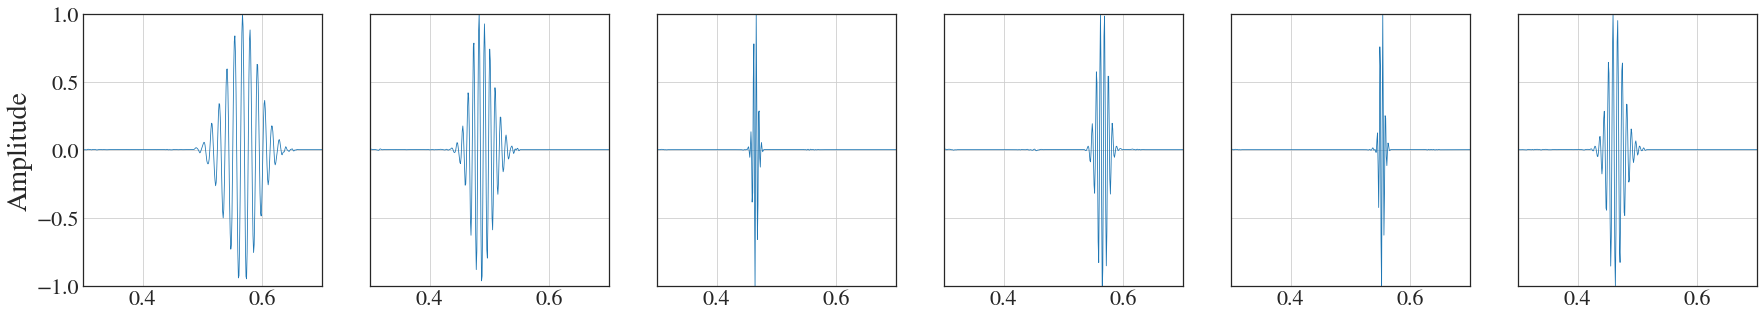
\includegraphics[width=\textwidth]{figures/generations/sg.png}
    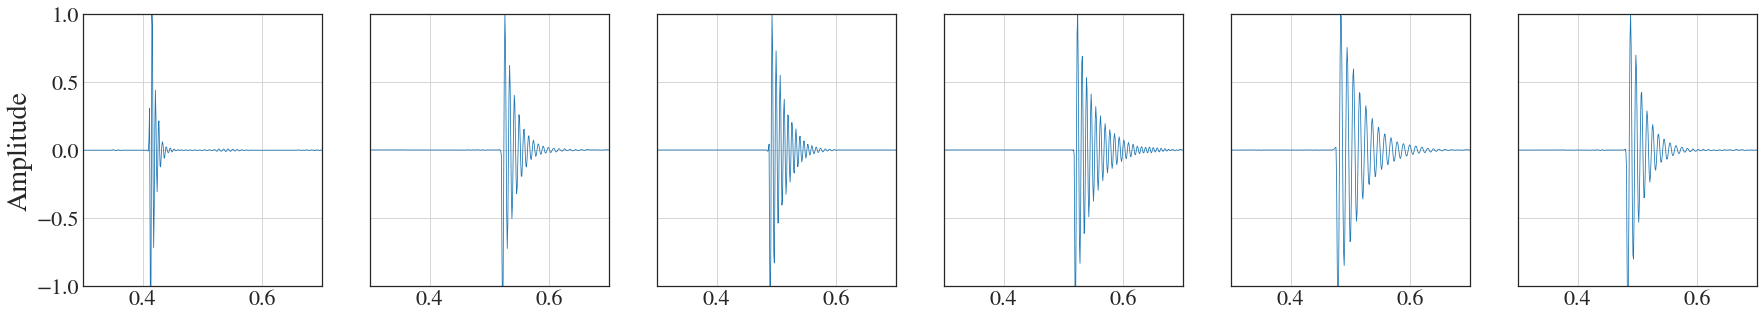
\includegraphics[width=\textwidth]{figures/generations/rd.png}
    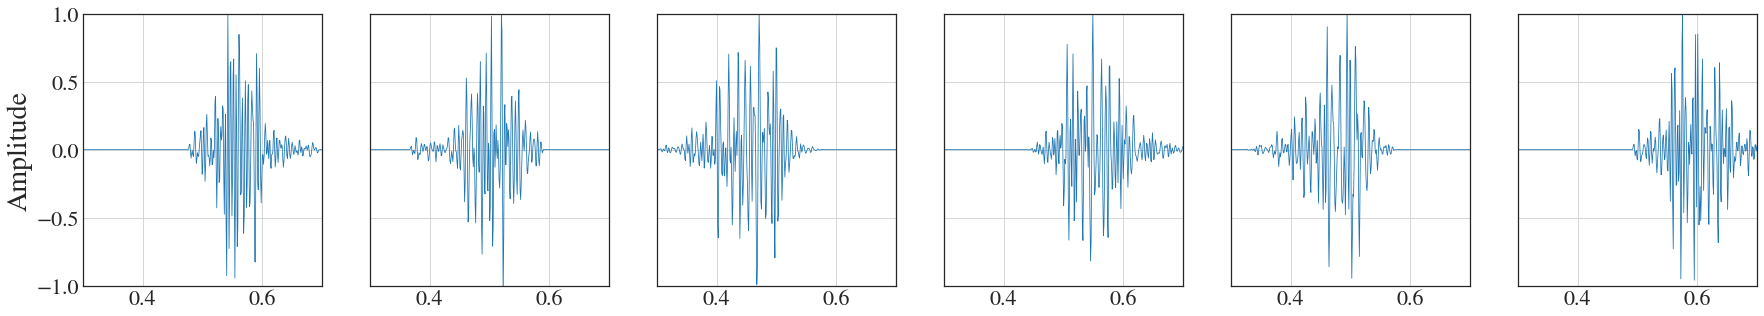
\includegraphics[width=\textwidth]{figures/generations/wnb.png}
    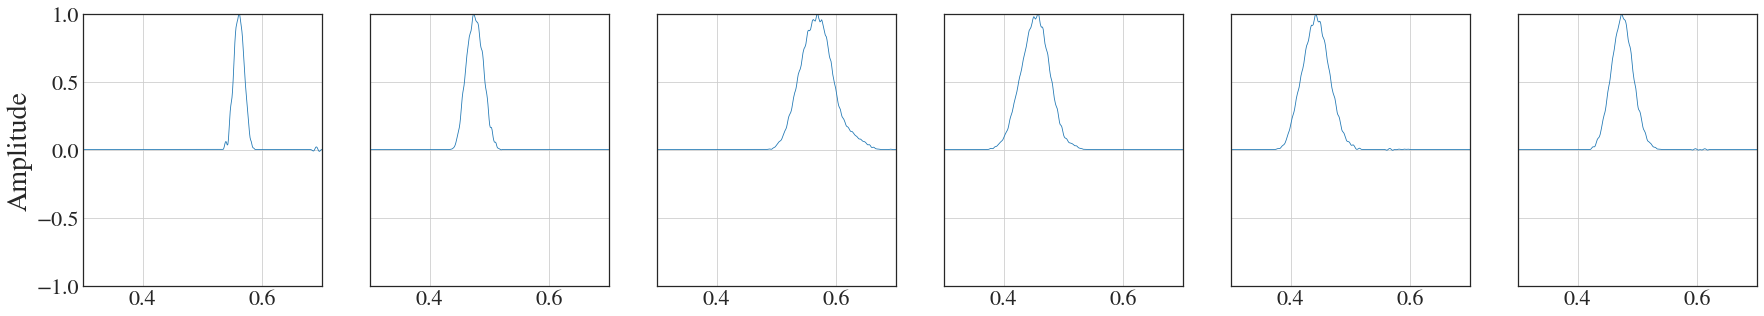
\includegraphics[width=\textwidth]{figures/generations/blip.png}
    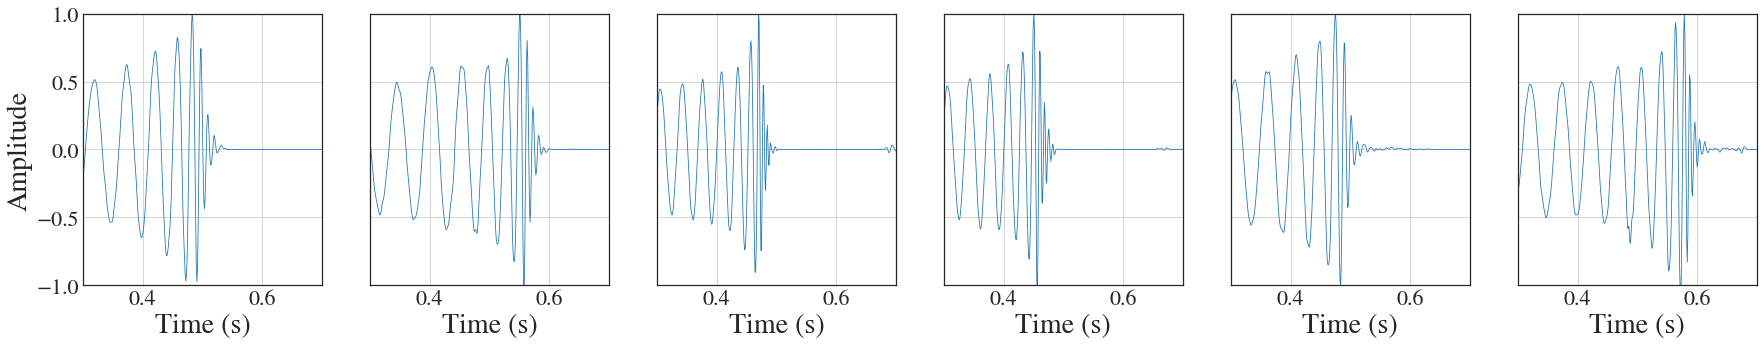
\includegraphics[width=\textwidth]{figures/generations/bbh.png}
    \caption{Examples of \ac{GW} burst signals generated by a conditional generative adversarial network. By row: Sine-Gaussian, Ringdown,
White-noise burst, Gaussian pulse, Binary black hole merger.}
\label{fig:gen_signals} \end{figure}

\subsection{Waveform quality}
The generator network is a function G : $\mathbf{z},\mathbf{c},\mathbb{\textbf{s}}$ $\in$ $\mathbb{R}^{100}$ $\to$ $\mathbb{R}^{1024\times2}$, where $\mathbf{z},\mathbf{c},\mathbb{\textbf{s}}$ are the latent vector, class embedding vector and sky positions respectively. Given a latent vector randomly sampled from a normal distribution with zero mean and unit variance, a class label which is represented by a 5 dimensional one-hot encoded vector for each class, the results from the generator can be seen in \cref{fig:gen_signals}. Each plot shows the output of the generator after given randomised $\mathbf{z}$ and one of the five class vectors $\mathbf{c}$.
 %Depending on the orientation of the detector with respect to a hypothetical signal in the sky, the waveforms may appear inverted, shifted in time and their strain attenuated. 

\subsection{Interpolation}
Machine learning algorithms are often described as universal function approximators. In the generators case it maps samples drawn from a 100 dimensional Gaussian space to its representation of the training set. As with any function, there should be a one to one mapping from the domain and co-domain to allow for smooth transitions across the latent space. One advantage of using GANs as a waveform generator is that once it is trained, it can perform rapid generations faster than computationally expensive algorithms. For complicated data sets, the network architecture must be diverse and dense enough to capture distinct variations from the training set. Most GANs perform well on relatively low resolution image generations, however, higher resolutions demand larger networks and long training times. GANs attempting to replicate complicated structures and do not have the necessary architecture either struggle to produce results at all or fall into the common failure mode know as mode collapse; where the generator produces a small variety of samples or simply memorises the training set. To test this, we perform linear interpolations in the latent and class space. 

\subsubsection{Latent space interpolation}
In this section we explore the latent space formed by the generator by interpolation. We take two random points in the latent space and linearly interpolate between them. These new latent space vectors can now be fed into the generator to make predictions on while keeping the class vectors constant. The full effect shown in \cref{fig:z_interp}. We can see that each plot shows plausible waveforms suggesting that the generator has constructed a smooth space unlike the discrete training case. Additionally as each class is given the same latent points to interpolate over, we can see that the waveforms cluster together with respect to their parameters. Visually, the sine-gaussian and ring-down waveforms share similar frequencies and the other signals show similar decays and starting epochs. The only exception is BBH waveforms, which is expected as they were trained with more variety of parameters and consistently have their peaks in the last quarter of the time series.

\begin{figure}
    \centering
    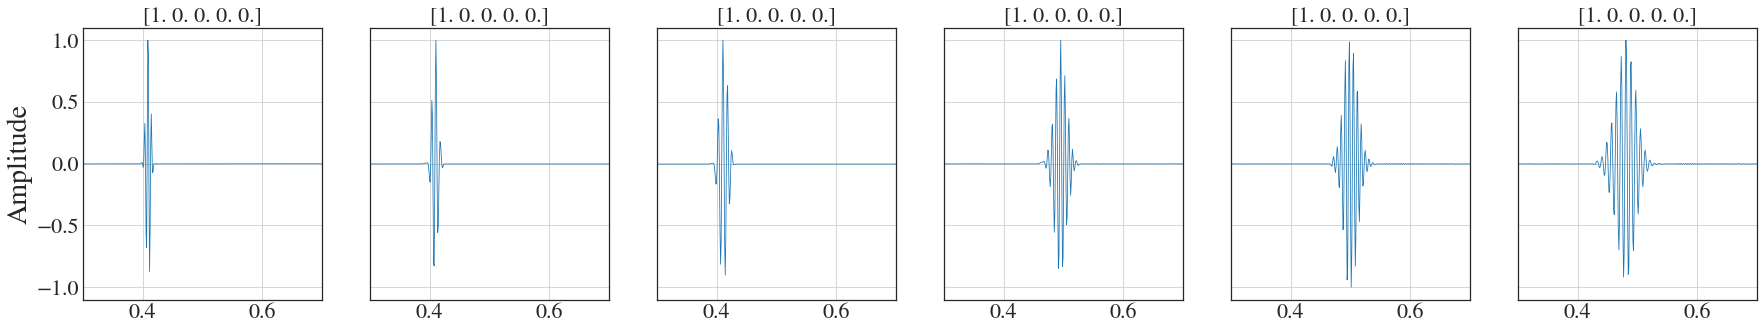
\includegraphics[width=\textwidth]{figures/generations/z_interp_sg.png}
    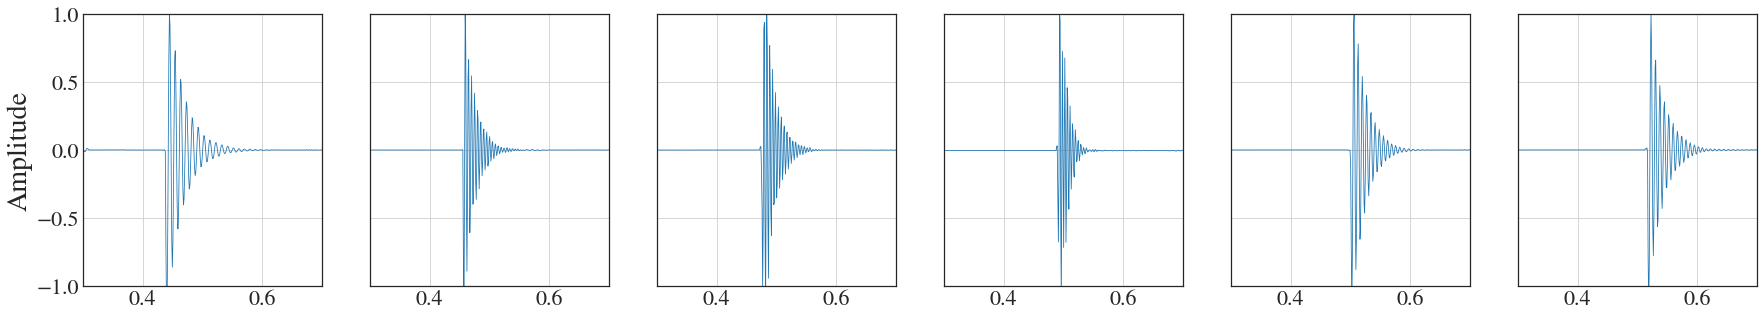
\includegraphics[width=\textwidth]{figures/generations/z_interp_rd.png}
    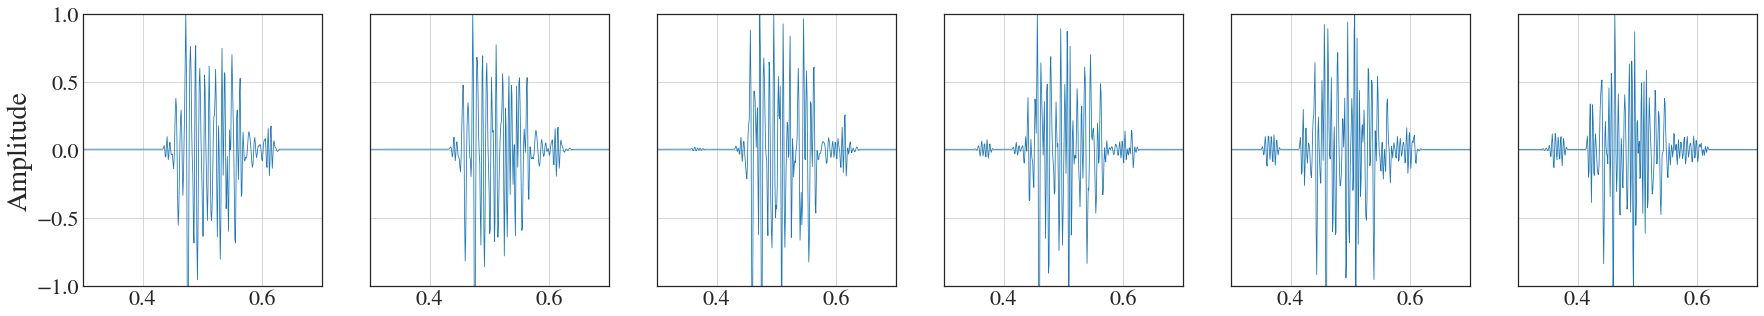
\includegraphics[width=\textwidth]{figures/generations/z_interp_wnb.png}
    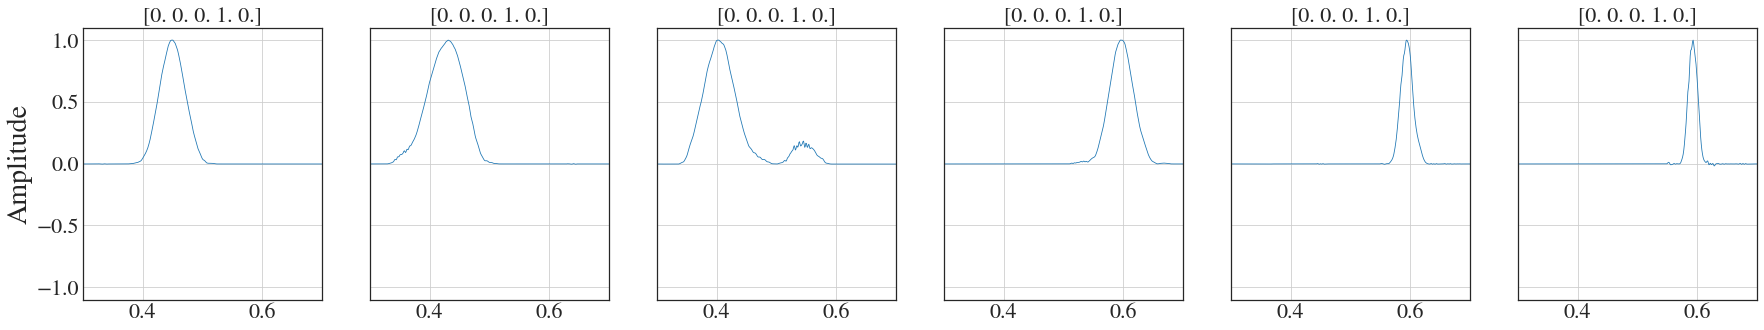
\includegraphics[width=\textwidth]{figures/generations/z_interp_blip.png}
    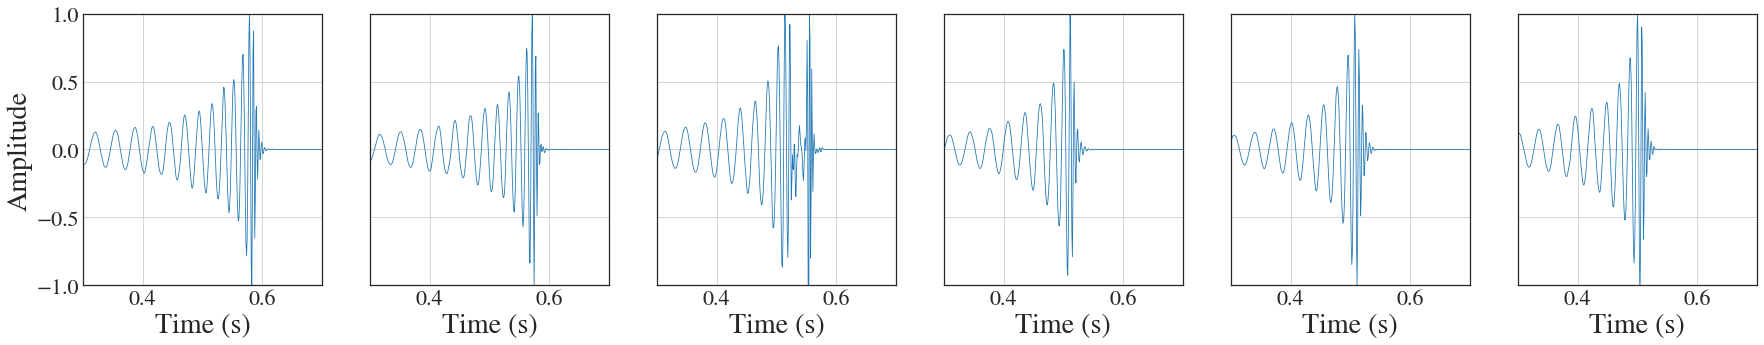
\includegraphics[width=\textwidth]{figures/generations/z_interp_bbh.png}
    \caption{Latent space linear interpolation, class space is held constant.}
    \label{fig:z_interp}
\end{figure}

\subsubsection{Class space interpolation}
In order to explore the class space we keep the latent vector held constant and interpolate through the 5 classes. We construct a path between the 5 waveforms and show that the space is populated enough to allow for transitions between classes. Sine-Gaussian to ringdown performs well in interpolation with each signal being a plausible burst GW. It is obvious that the GAN has clustered these two groups during training as they share many characteristics. The other signals have sharper transitions but still retain plausible looking waveforms. 

\begin{figure}
    \centering
    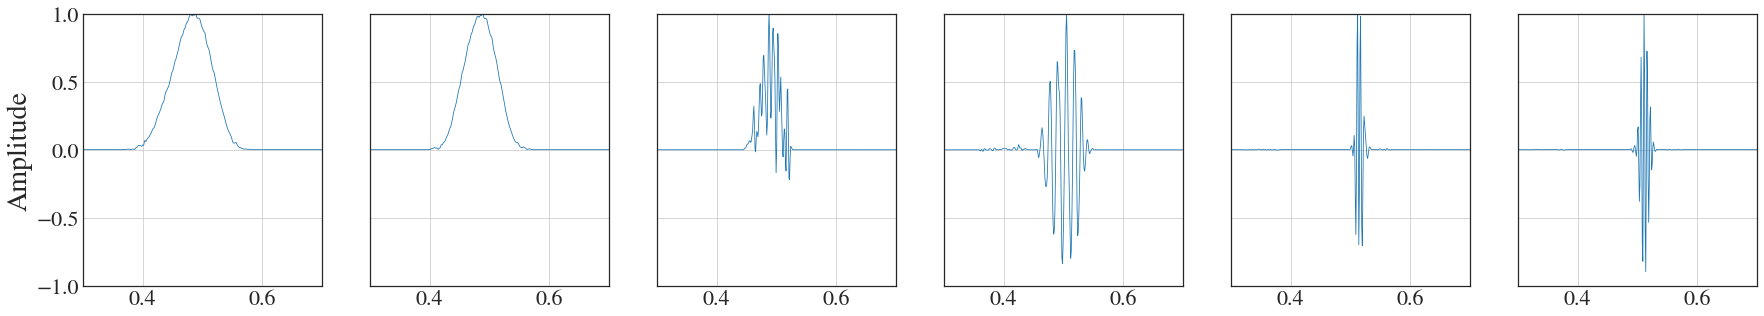
\includegraphics[width=\textwidth]{figures/generations/interp_blip-sg.png}
    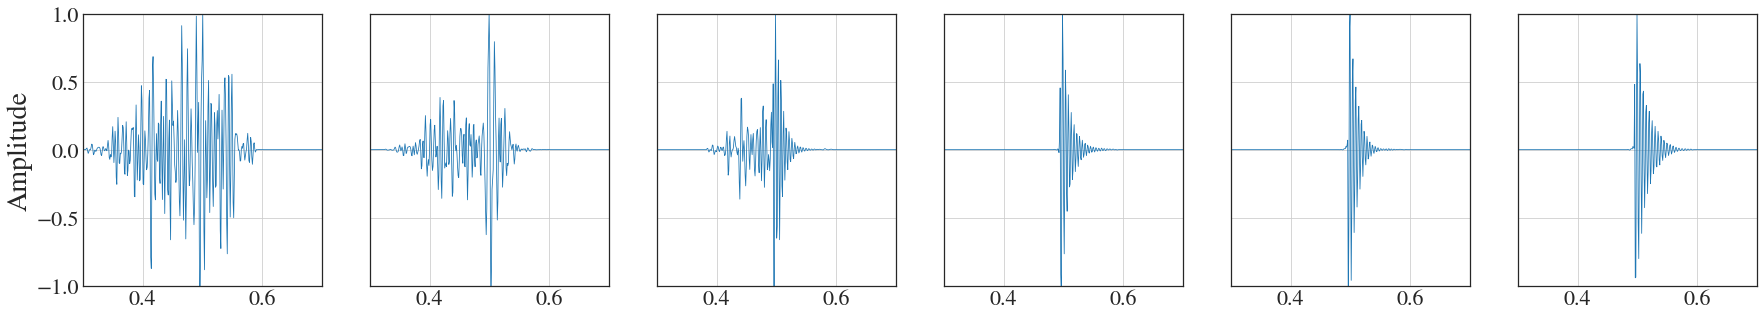
\includegraphics[width=\textwidth]{figures/generations/interp_wnb-rd.png}
    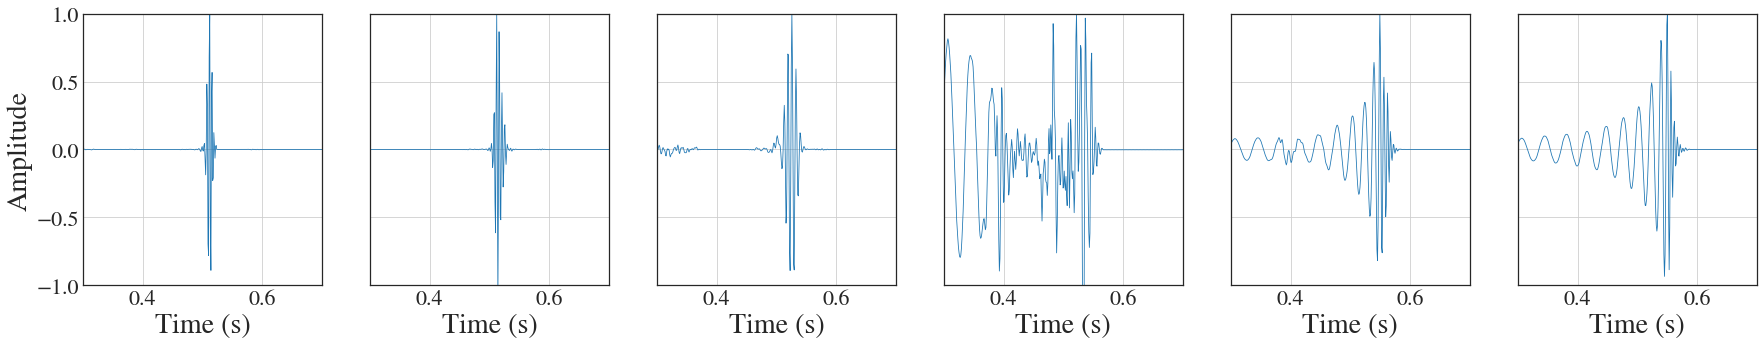
\includegraphics[width=\textwidth]{figures/generations/interp_sg-bbh.png}
    \caption{Class space linear interpolation, class space is held constant. Top row: gaussian blip to sine-gaussian, middle row: white noise burst to ringdown, bottom row: sine-gaussian to BBH.}
    \label{fig:c_interp}
\end{figure}

\subsection{Using a GAN to generate unmodelled waveforms}
So far the analysis has focused on interpolating between two classes of signals with the aim to use the interpolated signals as unmodelled waveforms, instead, we may consider random mixtures of classes. We defined the classes in one-hot encoding framework, that is, each class resides at the corner points of a 5 dimensional cube. In order to generate an even mixture of classes we sample points uniformly in this space. \jordan{this would be the box}. Alternativly we can sampe points from the plane that intersects the four corners, which for a 5-dimensional case is, sample from a 4-simplex. Thks can nbee seen in \ref{fig:unmodelled_samples}. \jordan{why? this enforces the vector points to sum to one. Why is that good? Well it keeps the points lying on the simplex.} 

\begin{figure}
    \centering
    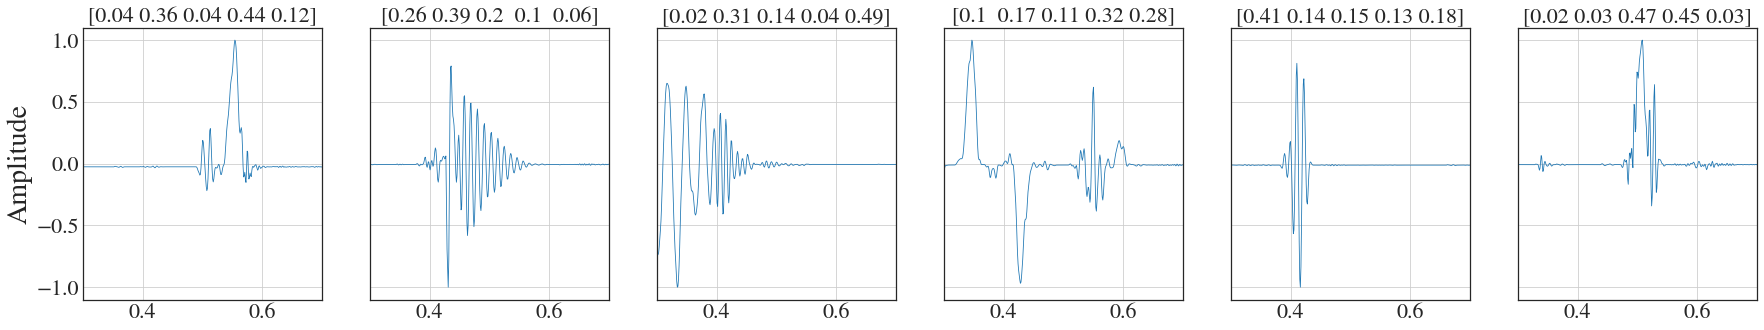
\includegraphics[width=\textwidth]{figures/generations/simplex_sample1.png}
    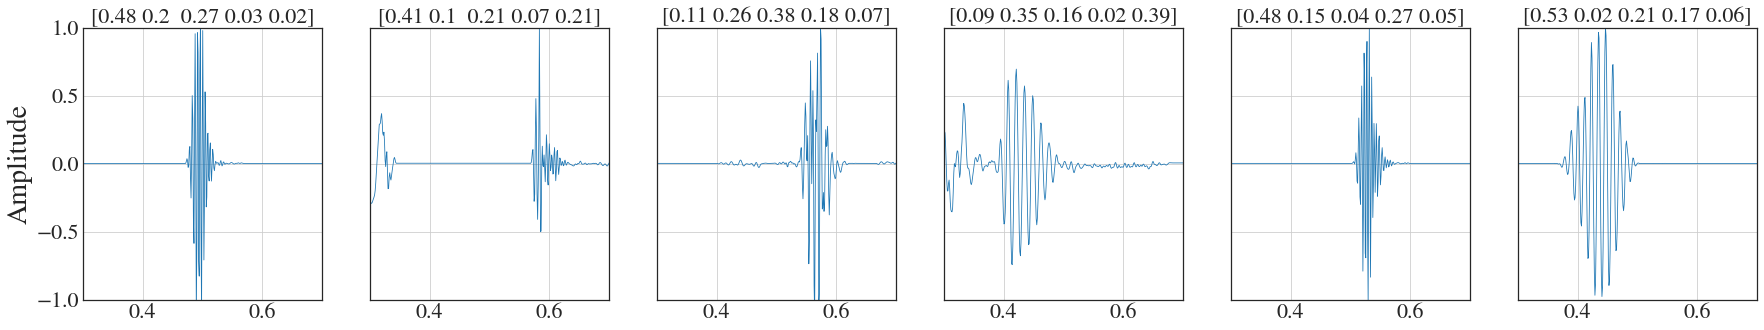
\includegraphics[width=\textwidth]{figures/generations/simplex_sample2.png}
    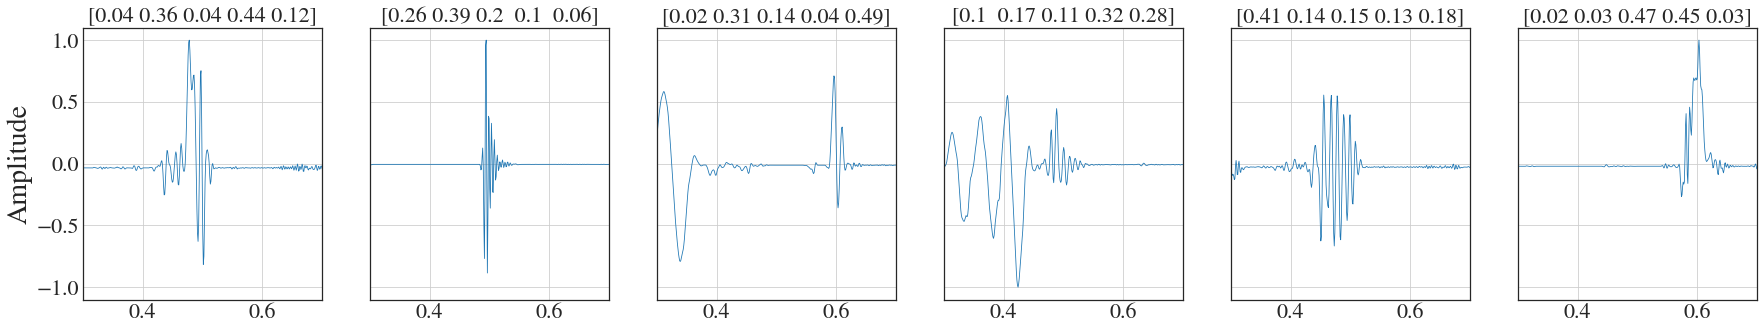
\includegraphics[width=\textwidth]{figures/generations/simplex_sample3.png}

    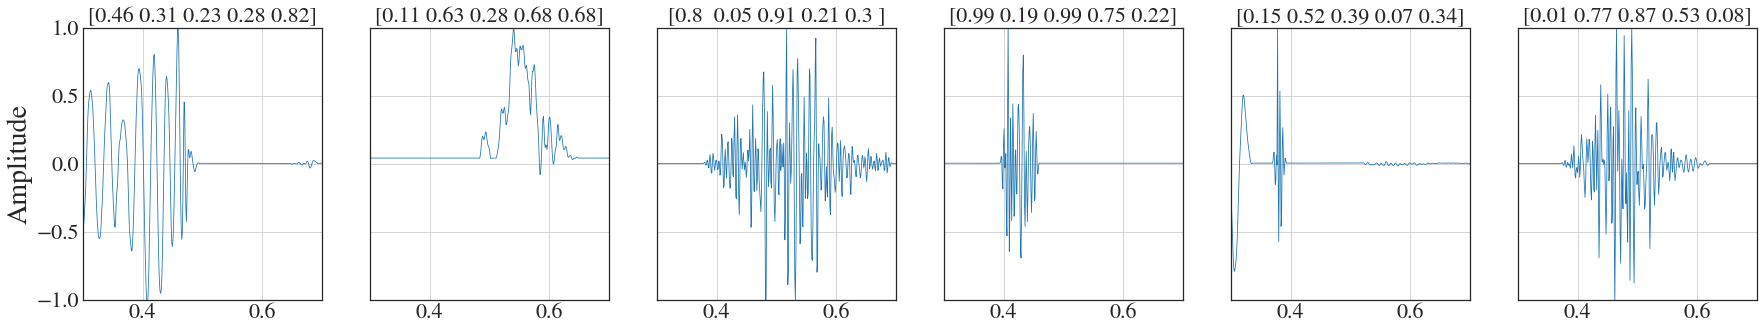
\includegraphics[width=\textwidth]{figures/generations/uniform_sample3.png}
    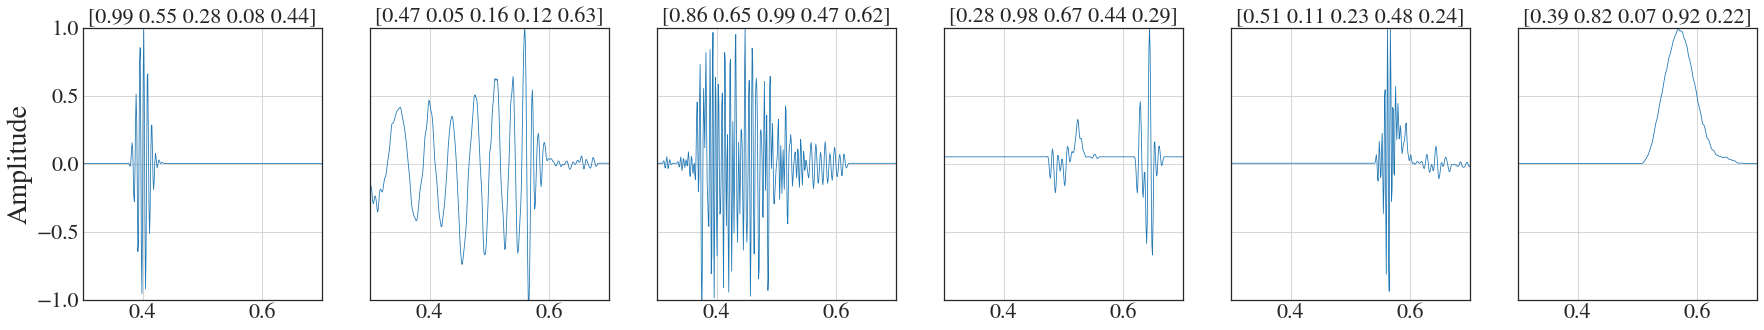
\includegraphics[width=\textwidth]{figures/generations/uniform_sample2.png}
    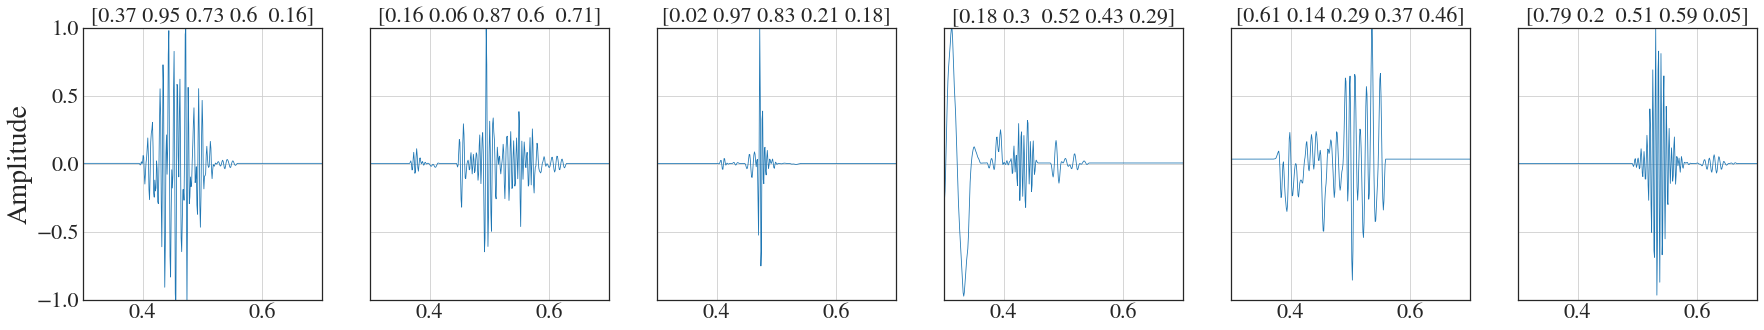
\includegraphics[width=\textwidth]{figures/generations/uniform_sample1.png}
    \caption{GAN generations where the class vectors are sampled from the 4-D plane and sampled uniformly in the class space.}
    \label{fig:unmodelled_samples}
\end{figure}


\begin{comment}
We can now think of ways to properly sample from the space between these points in a uniform way. Uniformity enforces the condition that we have a variety of waveforms. Thge easiest being to uniformly sample points in this space and use them as the class vectors for the generator. Another way would be to keep the magnitude of the class vector as 1. For a 5-dimensional space we would sample from the 4-dimensional plane that intersects the corner points. 
\end{comment}

\subsection{CNN analysis}
In this section of the analysis we will forensically compare generations from the GAN to help determine the success and failures of the model. We investigate a simple case of using a CNN to detect whether a signal is contained in noise or if the data is noise only. The signals we train the CNN on are generated from the GAN with their latent input randomised from a 100-dimensional Gaussian distribution and are categorised by their method of defining their class vector: 
\begin{itemize}
	\item Conditional – Definite categorical generations from the GAN. These signals are the closest to the training set.
	\item Uniform – Generated using a uniform distribution U[0,1] as the input class vector.
	\item Simplex – Generated using a Dirichlet distribution that samples from the 4-simplex as the input class vector. 
\end{itemize}
The CNN is trained to distinguish between two classes: signals in additive Gaussian noise and Gaussian noise, where “signals” are taken from either the Conditional, Uniform or Simplex cases. This means in total there are three CNNs to train and all CNNs share the same architectural structure. All of the training data used is “whitened” by a power spectral density (PSD) at Advanced LIGO design sensitivity, such that, there is equal power at each frequency and is correctly normalised. This procedure is applied to signals whose signal-to-noise ratios (SNRs) are defined prior to be in the range uniformly [1-16]. For each run the training data consists of 200,000 signals which contain one half noise only and one half signal contained in noise. Of that 80\% is used for training and 20\% used for validation. A different testing set is also used in analysis that is 200,000 in size. 

*table of parameters used for CNN*

In Fig. \ref{fig:roc_curves} we compare the CNN results between the three datasets, we train three CNNs on the Conditional, simplex and uniform data sets and use these models to make predictions on the other unseen datasets. We make a comparison by fixing the fraction of samples incorrectly identified as signals (false alarm rate) and plotting this versus the optimal SNR of the signals. 

\begin{figure}
    \centering
    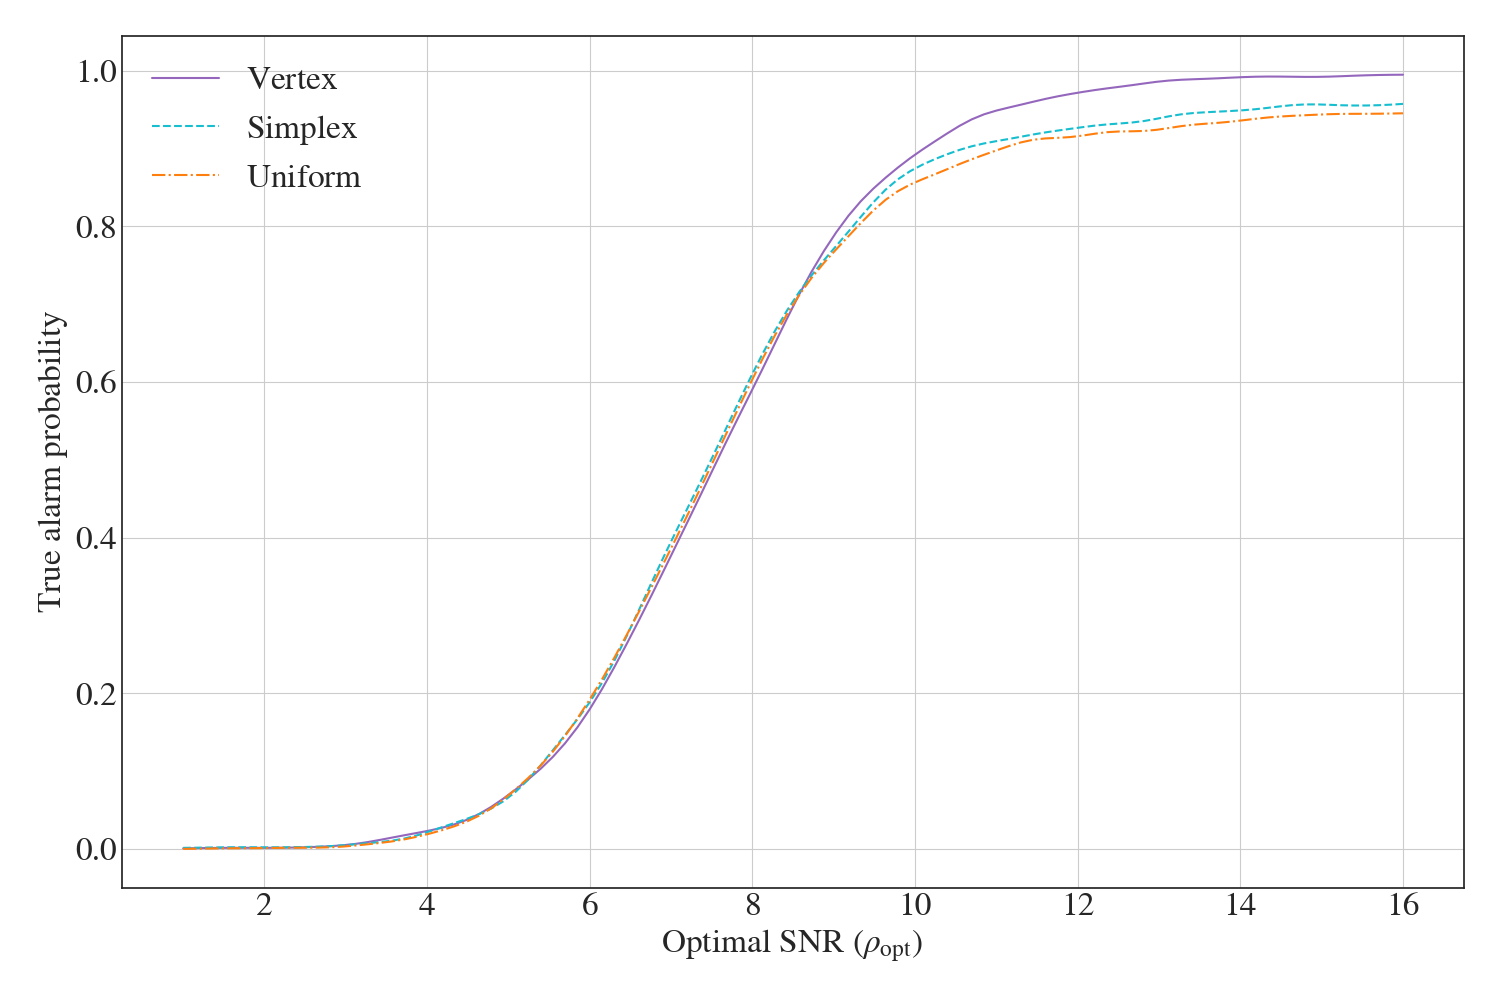
\includegraphics[width=0.8\textwidth]{figures/conditional_trained.png}
    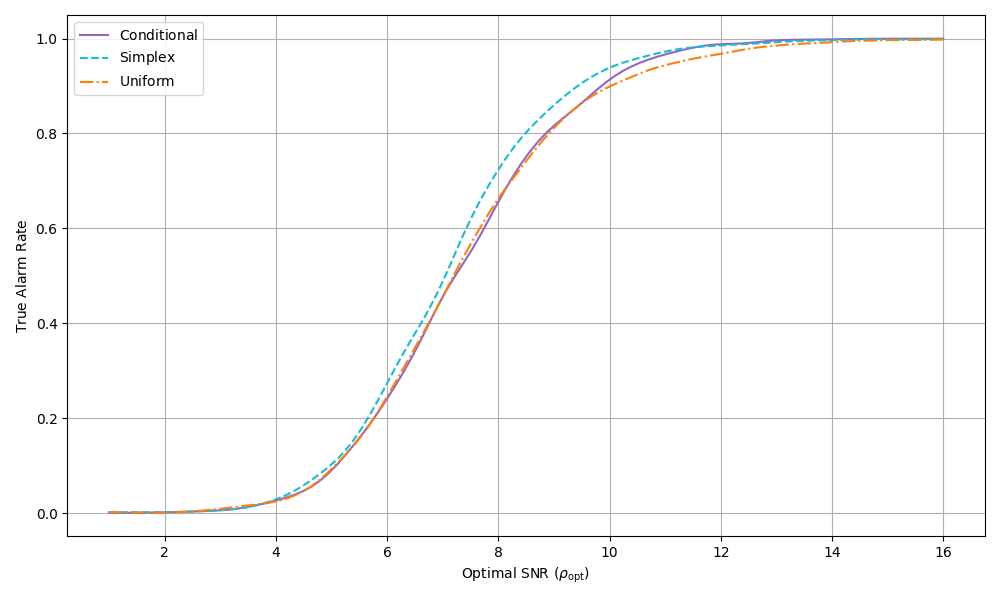
\includegraphics[width=0.8\textwidth]{figures/simplex_trained.png}
    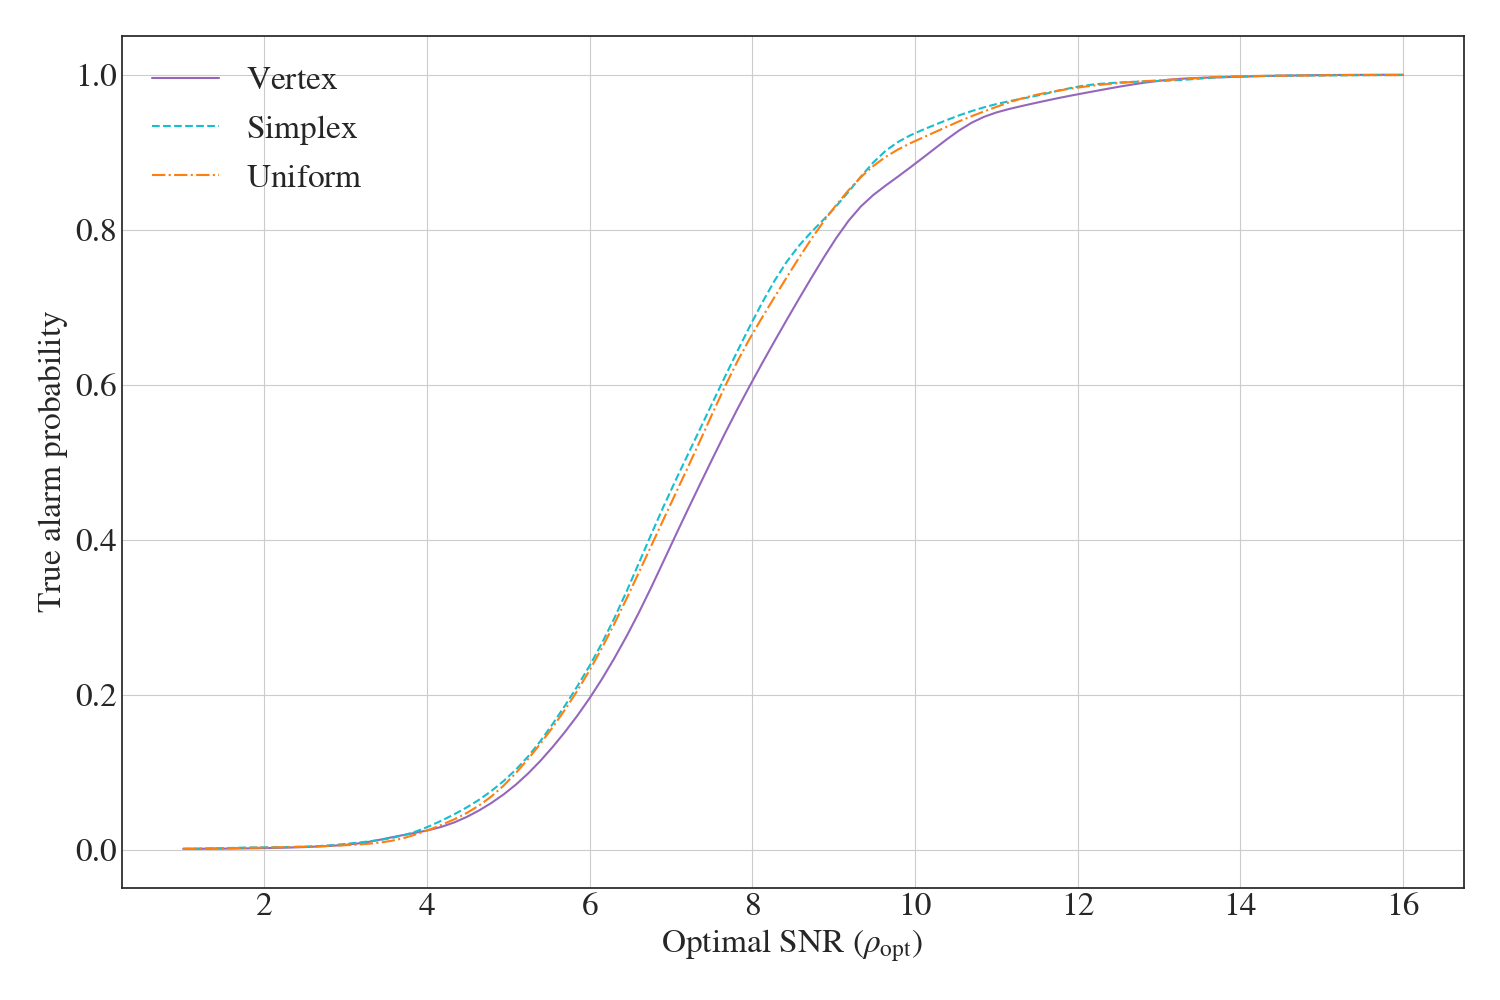
\includegraphics[width=0.8\textwidth]{figures/uniform_trained.png}

    \caption{Efficiency curves comparing the performance of CNNs trained on conditional generations (top), simplex generations (middle), uniform generations (bottom) for a fixed false alarm rate of $10^{-3}$.}
    \label{fig:roc_curves}
\end{figure}

These results show for a CNN trained on conditional signals, the uniform data set is distinguishable from the conditional and simplex dataset. The CNN is robust enough to capture the differences between the datasets and shows that the GAN can generate a variety of unmodelled waveforms that can be used in future testing. 

\begin{comment}
{\subsection{Vector Arithmetic}
In DCGANs the authors demonstrated unsupervised vector arithmetic with celebrity face generation. They kept points in the latent space and performed simple vector arithmetic to generate new images. This allows for intuitive and targeted generation of images. However, the authors realised that single images vectors were unstable and there was a need to average three vectors before any arithmetic. DCGANs is unconditional, therefore, the vectors used were chosen empirically, generating many faces and choosing the attributes for study. Here, we show that this GAN only needs a single vector representation and due to conditioning we can have more control over which vectors to use in the arithmetic. In \cref{fig:arithmetic} we generate a whitenoise burst and a BBH insprial using their respective class labels and use a randomised latent point and response. Keeping the latent point and response, we average the two class vectors and use this as input to the generator. \Cref{fig:arithmetic} (c) shows the generation based on the combined class vectors which visually looks similar to a supernova waveform. Supernova waveform generations require expensive numerical relativity simulations and various assumptions about the collapse of its parent star. Here, we are able to produce similar waves at a fraction of the expense and we are able to further modify the resultant by using different latent space samples. \jordan{this is the adding noise thing but i need to work out the correct way to do it with the directional vector}. 
\end{comment}



%%%%%%%%%%%%%%%%%%%%%%%%%%%%%%%%%%%%%%%%%%%%%%%%%%%%%%%%%%%%%%%%%%%%%%%%%%%%%%
\section{Conclusions}
%%%%%%%%%%%%%%%%%%%%%%%%%%%%%%%%%%%%%%%%%%%%%%%%%%%%%%%%%%%%%%%%%%%%%%%%%%%%%%
In this work we present the potential of Generative Adversarial Networks for burst gravitational wave analysis. We have shown that GANs have the ability to generate 5 class varieties of modelled burst \ac{GW} signals that can be generated at whim. The latent and class spaces were explored through interpolation and suggest that the space provides smooth translations between classes and overall waveform shape. We then showed targeted waveform generation by mixing classes to produce new unmodlled waveform varieties that can be used to test current burst search pipelines. \jordan{couple of sentences about classifier}. 

In order to extend this work to a viable burst wave generator and classifier a few points require further research. In principle it is trivial to add another detector inside the response layer \jordan{response is the wrong thing to say since the time delay isnt really a response, extrinsic layer? just non trainable layer? The box?}, however, as this now 3 dimensional signal is feed to the discriminator this will no doubt require further tweaking of the network. We can add more burst-like wave forms in the training set, like detector glitches which would similarly require further network design. The work presented here is noise free. To havea complete generation and detection package we would like to train the network on signals hidden in additive Gaussian noise and test the ability of the auxiliary classifier. 

The approach shown in this work shows promise in generating unmodelled burst waveforms from exotic sources. Having the ability to quickly generate new waveforms is essential to test current detection schemes and their susceptibilty to unmodelled sources. We belive that GANs have the ability to generate high fidelity waveforms at a fraction of the computational expense and do not rely on large prior parameter space. Having banks of these waveforms at hand can aid in our understand of the physics processes behind these non-standard gravitational wave emitters.  

\jordan{I want to include a link to the github etc but also a google collab scrip like the one for BigGANs: \\
\url{https://colab.research.google.com/github/tensorflow/hub/blob/master/examples/colab/biggan_generation_with_tf_hub.ipynb.} 
It's fun and gives a better feel for the interpolating that static images.}

\begin{comment}
\begin{itemize}
\item Summarise the paper
\item Dedicate a paragraph to each of the key results discussed in the previous
section
\item Have at least one paragraph on the future directions of this work
\item Conclude with a positive paragrpah about the potential uses and impact of
the approach.
\end{itemize}
\end{comment}

\section*{References}
\bibliography{iopart-num}

\clearpage

\appendix
\section{List of hyperparameters}
\begin{table}[hb]
\caption{ACGAN architecture}
\footnotesize
\begin{tabular}{@{}l l l l l l l}
\br
 Operation & Kernel & Strides & Output Shape & BN & Dropout & Activation \\
\mr
 G(\textbf{z}): Input \textbf{z} $\sim$ Normal(0,0.02) & N/A & N/A & (100,) & \ding{55} & 0 & N/A \\  
 Dense & N/A & N/A & (32768,) & \ding{55} & 0 & ReLU \\  
 Class input c & N/A & N/A & (1,) & \ding{55} & 0 & N/A \\
 Embedding & N/A & N/A & (1, 120) & \ding{55} & 0 & N/A \\
 Dense & N/A & N/A & (1,128) & \ding{55} & 0 & ReLU \\ 
 Reshape \textbf{z} & N/A & N/A & (128, 256) & \ding{55} & 0 & N/A \\
 Reshape c & N/A & N/A & (128, 1) & \ding{55} & 0 & N/A \\
 Concatenate & N/A & N/A & (128, 257) & \ding{55} & 0 & N/A \\
 Reshape & N/A & N/A & (64, 514) & \ding{55} & 0 & N/A \\
 Transposed Convolution & 18x1 & 2 & (256, 256) & \ding{51} & 0 & ReLU\\
 Transposed Convolution & 18x1 & 2 & (512, 128) & \ding{55} & 0 & ReLU\\
 Transposed Convolution & 18x1 & 2 & (1024, 64) & \ding{55} & 0 & ReLU\\
 Convolution & 18x1 & 1 & (1024, 1) & \ding{55} & 0 & Tanh \\
 Sky input & N/A & N/A & (3,) & \ding{55} & 0 & N/A \\
 Concatenate & N/A & N/A & (1027,) &  \ding{55} & 0 & N/A \\
 Lambda & N/A & N/A & (1024, 2) & \ding{55} & 0 & N/A \\
 D(\textbf{x}): Input \textbf{x} & N/A & N/A & (1024, 2) & \ding{55} & 0 & N/A \\
 Convolution & 14x1 & 2 & (512, 64) & \ding{55} & 0.5 & Leaky ReLU \\
 Convolution & 14x1 & 2 & (256, 128) & \ding{55} & 0.5 & Leaky ReLU \\
 Convolution & 14x1 & 2 & (128, 256) & \ding{55} & 0.5 & Leaky ReLU \\
 Convolution & 14x1 & 2 & (64, 512) & \ding{55} & 0.5 & Leaky ReLU \\
 Flatten & N/A & N/A & (32768,) & \ding{55} & 0 & N/A \\
 Dense & N/A & N/A & (1,) & \ding{55} & 0 & Sigmoid \\
 Dense & N/A & N/A & (5,) & \ding{55} & 0 & Softmax \\
\br
 Optimizer & \multicolumn{6}{l}{Adam($\alpha$ = 0.0002, $\beta_{1}$ = 0.5)} \\
 Batch size & \multicolumn{6}{l}{128}  \\
 Iterations & \multicolumn{6}{l}{60000}  \\
 Leaky ReLU slope & \multicolumn{6}{l}{0.2} \\
 Weight initialization & \multicolumn{6}{l}{Gaussian($\mu$ = 0, $\sigma$ = 0.02)} \\
 Generator loss & \multicolumn{6}{l}{Binary cross-entropy} \\
 Discriminator loss & \multicolumn{6}{l}{Binary cross-entropy \& sparse categorical cross-entropy} \\ 
 \br
\end{tabular}\\
\label{Tab:hyperparameters}
\end{table}
\normalsize

\section{Many more generated examples}

\end{document}

